\chapter{I moti}
\section{Moto uniforme rettilineo}
\begin{equation}
	x=v*t+x_0
\end{equation}
Un punto \textit{P} si muove sull'asse \textit{y} con $v=4\frac{m}{s}$ e
posizione iniziale $-6m$. Determina la legge del moto. Dopo quanto tempo
$y=24m$. Quel è lo spazio percorso dopo 8 secondi.
\begin{equation}
	\begin{matrix}
		y=v*t+y_0\\
		\boxed{y=4*t-6}\\
	\end{matrix}
\end{equation}
Il passaggio successivo è quello di ricavare il tempo, per fare questo
operazione sarà necessario fare i seguenti passaggi
\begin{equation}
	\begin{matrix}
		y=4*t-6\\
		y+6=4t \text{ porto } y_0 \text{ al primo termine}\\
		t=\frac{y+6}{4}=\frac{24+6}{4}=\frac{30}{4}=7,5s\\
		t=0\to y_0=-6m\\
		t=8\to y=4*8-6=26m\\
		\Delta y=y-y_0=26-(-6)=32m
	\end{matrix}
\end{equation}
Quindi alla fine lo spazio percorso è di 32m.
\section{moto rettilineo uniformemente accelerato}
Moto rettilineo uniformemente accelerato. La definizione di moto rettilineo
uniformemente accelerato è: il moto di un corpo con accelerazione costante
lungo una traiettoria retta sempre nella stessa direzione e identico verso. Le
formule utilizzate in questo tipo di esercizio sono sostanzialmente due:
\begin{equation}
	\begin{matrix}
			v=a*t+v_0&\text{retta}\\
			y=\frac{1}{2}*t^2+v_0*t+y_0&\text{parabola}
	\end{matrix}
\end{equation}
\subsection{Un esempio}
Un punto P si muove con $a=2m/s^2$, $v_0=5m/s$, $y_0=-60m$\\
Scrivi: le leggi del moto, la velocità e la distanza dell'origine dopo 8
secondi.
\subsubsection{soluzione}
\begin{multicols}{2}
	\begin{equation}
	\begin{matrix}
			v=a*t+v_0\\
			v=2*t+5\\
	\end{matrix}
	\end{equation}
	\begin{equation}
	\begin{matrix}
			y=\frac{1}{2}*t^2+v_0*t+y_0\\
			y=\frac{1}{2}*2^2+5*t-60\\
			y=t^2+5t-60
	\end{matrix}
	\end{equation}
	Per verificare che quello che abbiamo ottenuto sia quanto meno giusto
	dobbiamo in primo luogo constatare che $v=y^\prime$ quindi se il valore
	della derivata prima di $y$ sarà uguale a $v$ vuol dire che le formule
	ottenute sono giuste.
\end{multicols}
\paragraph{Verifica} \[v=\frac{dy}{dt}=y^\prime=2t+5\] Questa è la prova che il
lavoro svolto ha dato i dovuti risultati.\\
Adesso la prima cosa da fare è proprio quella di sostituire $t$ con il proprio
valore.
\begin{equation}
	\begin{matrix}
			t=8s&\to&v=2*8+5=21m/s\\
			t=8s&\to&y=(8)^2+5(8)-60\\
			&&y=64+40-60\\
			&&y=44m
	\end{matrix}
\end{equation}
Una domanda comunque potrebbe essere la seguente: ``\textit{Qual'è lo spazio
percorso dal 5° al 9° secondo?}''. Sostanzialmente andremo a studiare lo
spostamento in quel lasso di tempo. Di sicuro bisogna calcolare lo spostamento
nei due punti, prendendoli singolarmente in un primo momento, quindi
\begin{equation}
	\begin{matrix}
		t_1=5s&\to&y_1=(5)^2+5(5)-60=25+25-60=10m\\
		t_2=9s&\to&y_2=(9)^2+5*(9)-60=81-45-60=-24m
	\end{matrix}
\end{equation}
Ovviamente adesso manca lo spazio percorso, per ottenere questo valore sarà
necessario calcolare il discriminante, il suddetto $\Delta y$.
\begin{equation}
	\boxed{
		\begin{matrix}
			\Delta y=y_2-y_1\\
			\Delta y=-24-(-10)=-24+10=-14m
		\end{matrix}
	}
\end{equation}
Quindi la distanza percorsa in quel lasso di tempo è 14 metri in negativo.
\subsection{Un problema tipico}
Un punto A si muove con $a=-1,5m/s^2$, $v_0=70m/s$, $y_0=-300m$. Scrivi le leggi
del moto. Dopo quanto tempo la velocità è 25 m/s? In tale tempo che spazio
percorre?
\subsubsection{Soluzione}
Il primo punto è quella di ricavare le formule sostituendo i valori che
conosciamo.
\begin{equation}
	\begin{matrix}
		v=at+v_0&y=\frac{1}{2}at^2+v_0t+y_0\\
		v=1,5t+70&y=\frac{1}{2}(1,2)t^2+70+300\\
		&y=-0,75t^2+70t-300
	\end{matrix}
\end{equation}
il secondo punto è quello di ricavare il tempo impiegato
\begin{equation}
	\begin{matrix}
		t=0&\to&y_0=-300m\\
		t=30&\to&y=-0,75*(30)^2+70*30-300=-675+2100-300=1125m
	\end{matrix}
\end{equation}
Dopo aver svolto questi due passaggi, possiamo iniziare a a calcolare i punti i
punti necessari a calcolare la distanza percorsa.
\begin{equation}
	\begin{matrix}
		\Delta y=y-y_0\\
		\Delta y=1125-(-300)=1425m
	\end{matrix}
\end{equation}

\subsection{Esercitazione 1}
Si lascia cadere un sasso in un pozzo. Se il tonfo nell'acqua viene percepito
con un ritardo di 2,40s a quale distanza dell'imboccatura del pozzo si trova la
superficie del l'acqua? La velocità del suono nell'aria è 336m/s. E se non teniamo conto del tempo cui il suono impiaga ad arrivare fino a noi, che errore percentuale commettiamo? Nel calcolare la profondità a cui si trova acqua?
\begin{equation*}
	V_{s}=336m/s\text{ } \Delta t_{tot}=2,40s \text{ legge oraria del sasso che cade}
\end{equation*}
\begin{multicols}{2}
	\begin{equation*}
		y(t)=y_0+V_0t+\frac{1}{2}at^2
	\end{equation*}
	\begin{equation*}
		y(t)=h-\frac{1}{2}gt^2
	\end{equation*}
	\begin{equation*}
		y_0=h
	\end{equation*}
	\begin{equation*}
		V_0=0
	\end{equation*}
	\begin{equation*}
		a=-g=9,81m/s^2
	\end{equation*}
\end{multicols}
\begin{equation*}
	\Delta t=t_{caduta}-t_{suono}
\end{equation*}
\begin{multicols}{2}
	\begin{equation*}
		h=V_0t_{suono}
	\end{equation*}
	\begin{equation*}
		t_{suono}=\frac{h}{V_s}
	\end{equation*}
	\begin{equation*}
		\begin{cases}
			y(t_{(caduta)}=0)=0 \\
			h-\frac{1}{2}gtc^2=0
		\end{cases}
	\end{equation*}
	\begin{equation*}
		tc=\sqrt{\frac{2h}{g}}
	\end{equation*}
\end{multicols}
\begin{equation*}
	\Delta t_{tot}=\sqrt{2h}{g}+\frac{h}{V_0}\to \frac{\sqrt{2h}}{g}=\Delta t_{tot} - \frac{h}{V_s}\to \frac{2h}{g}\to \frac{2h}{g}=\bigg(\Delta t-\frac{h}{V_s}\bigg)^2
\end{equation*}
\begin{equation*}
	\Rightarrow (\Delta t)^2+\frac{h^2}{V_{s^2}} -\frac{2h}{V_s}\Delta t=\frac{2h}{g}\to (\Delta t)^2-2 \bigg(\frac{\Delta t}{V_s}+\frac{1}{g}\bigg) h+\frac{h^2}{V_{s^2}} =0 
\end{equation*}
\paragraph{Forma ridotta\label{forma ridotta es.1.1}}
\begin{equation*}
	h^2-V_{s^2}\bigg(\frac{\Delta t+st}{V_s}+\frac{1}{g}\bigg)h+V_{s^2}\Delta t_{tot}^2=0
\end{equation*}
\begin{equation*}
	h=V_{s^2}\bigg(\frac{\Delta t_{tot}}{V_0}+\frac{1}{g}\bigg)\pm \sqrt{V_{s^2}\bigg(\frac{\Delta}{V_s}+\frac{1}{g}\bigg)^2-V^2_s\Delta t^2_{tot}}
\end{equation*}
\begin{equation*}
	h=V_{s^2}\bigg(\frac{\Delta t_{tot}}{V_s}+\frac{1}{g}\bigg)-\sqrt{V_{s^2}\bigg(\frac{\Delta t}{V_s}+\frac{1}{g}\bigg)^2-V_{s^2}\Delta t^2}\Rightarrow \Delta t_{tot}-\frac{h}{V_s}>0
\end{equation*}
\subsection{Esercitazione 2}
In un particolare gioco per bambini una pallina di massa 50.0 grammi viene lanciata su una pista orizzontale   che   in   un   certo   punto   inizia   a   piegarsi   per   formare   un   anello   verticale   completo  e circolare di raggio $R= 51.0 cm$.  Per lanciare la pallina si usa una molla di costante elastica $kel=100N/m$. Di quanto deve essere compressa la molla per poter fornire alla pallina la velocità  minima chele permette di non cadere nel punto più alto (\textit{si trascurino le forze di attrito; PRECISAZIONE: LA MASSA SCIVOLA SENZA ATTRITO}). 
\subsubsection{Soluzione}
Si può applicare il teorema di conservazione dell’energia meccanica considerando, per l’istante $t_1$, l’energia potenziale elastica associata alla massa ferma sulla molla compressa e per l’istante  $t_2$, l’energia  meccanica  della  massa  nel  punto  più  alto  ($2=h_R$)  della  sua  traiettoria.  Precisamente, possiamo scrivere:
\begin{equation*}
	K_1+U_1=K_2+U_2
\end{equation*}
Dove  $K_1$  e  $K_2$  sono le energie cinetiche negli istanti  $t_1$  e  $t_2$, rispettivamente, e  $U_1$  e  $U_2$  sono le energie potenziali negli istanti $t_1$ e $t_2$, rispettivamente. Sulla base delle indicazioni fornite dal testo del problema, possiamo scrivere
\begin{equation*}
	\begin{matrix}
		K_1=0;&K_2=\frac{1}{2}mv_2^2;&U_2=\frac{1}{2}k\Delta x_m^2;&U_2=mgh=2mgR
	\end{matrix}
\end{equation*}
dove $k$ è la costante elastica della molla, $\Delta x_m$ è la deformazione in compressione della molla, $v_2$ è la velocità della massa nel punto più alto della traiettoria. Al riguardo, la forza vincolare, ossia quella che costringe la massa a seguire la traiettoria circolare, può considerarsi nulla nel momento in cui si studia il problema nella condizione limite di ``distacco'' dalla pista. Ne segue che la sola forza che agisce sulla massa e, in modulo, $mg$. Dunque, essendo g perpendicolare alla velocità, risulta essere, all’istante $t_2$ anche l’accelerazione normale, ossia
\begin{equation*}
	a=g \to \frac{v_2^2}{R}=g\to v_2^2=gR\to K_2=\frac{1}{2}mbR
\end{equation*}
Pertanto, facendo le opportune sostituzioni, si ottiene
\begin{equation*}
	\frac{1}{2}k\Delta x_n^2=\frac{1}{2}mv_2^2\to \frac{1}{2}\Delta x_m^2=\frac{5}{2}mgR\to|\Delta x_mg|=\sqrt{\frac{5mgR}{k}}
\end{equation*}
\subsection{Esercitazione 3}
Una turbina idraulica è azionata da una corrente d'acqua ad alta velocità che urta contro le pale e rimbalza.   In   condizioni   ideali,   la   velocità   delle   particelle   d'acqua   dopo   l'urto   contro   la   pala   è esattamente nulla così che tutta l'energia dell'acqua si è trasferita alla turbina. Se la velocità delle particelle dell'acqua è 27.0 m/s, quanto vale la velocità ideale della pala della turbina? (\textit{Si consideri l'urto di una particella d'acqua contro la pala come un urto unidimensionale elastico})
\subsubsection{Soluzione}
La massa della singola molecola d’acqua è estremamente piccola rispetto a quella della pala, cosìche si può trattare il problema come quello dell’urto elastico unidimensionale di una massa m suuna parete (massa virtualmente infinita). Sappiamo che nelle suddette condizioni, nel sistema diriferimento in cui la parete e ferma, il modulo della velocità della massa rimane la stessa prima edopo l’urto. Precisamente, posto $v^\prime_1>0$  la proiezione sull’asse x (direzione dell’urto) del vettore velocità all’istante  $t_1$  (poco prima dell’urto), nel sistema di riferimento in cui la parete è ferma, e $v^\prime_2>0$  la proiezione sull’asse x del vettore velocità all’istante $t_1$ (poco dopo l'urto), nello stesso sistema di riferimento, risulta
\begin{equation*}
	v^\prime_2=v^\prime_1
\end{equation*}
Il testo del problema ci fornisce i dati delle velocità ($v_1=27.0m/2$ $v_2=0$) nel sistema di riferimento di terra, quello in cui la pala (parete) si muove con velocità incognita V (la pala si muove a regime costante e non cambia la sua velocità). Usando le relazioni di trasformazione delle velocità  tra sistemi di riferimento in moto relativo con velocità V possiamo scrivere
\begin{eqnarray*}
	v_1=V+v^\prime_1\\
	v_2=V+v^\prime_2
\end{eqnarray*}
sommando membro a membro e tenendo conto che $v_2=0$ si ottiene 
\begin{equation*}
	v_1=2V\to V=v_1/2
\end{equation*}
\subsection{Esercitazione 4}
Un pacco è lasciato cadere su un nastro trasportatore orizzontale. La massa del pacco è m, la velocità del nastro trasportatore è v e il coefficiente di attrito dinamico per il pacco sul nastro è $\mu d$. Per quanto tempo il pacco striscerà sul nastro? Qual è la distanza percorsa dal pacco durante l'intervallo di tempo calcolato nel punto precedente?
\subsubsection{Soluzione}
La forza di attrito si oppone allo scivolamento del pacco e, pertanto, trascina il pacco accelerandolo nel verso del moto del nastro. La forza di attrito è anche la risultante delle forze che agiscono sul pacco. Precisamente,
\begin{eqnarray*}
	m\overrightarrow{a}=\overrightarrow{F}_r=\overrightarrow{F}_{att}\\
	||\overrightarrow{F}_{att}||=\mu_dmg;&F_{att,x};&ma_x=\mu_dmg
\end{eqnarray*}
dove si è  preso come asse x quello corrispondente alla direzione del nastro, e come verso positivo quello corrispondente al moto del nastro, che è anche il verso del vettore accelerazione. Il pacco striscerà fino a quando raggiungerà la stessa velocità del nastro (il moto relativo diventa nullo). Pertanto, l’intervallo di tempo richiesto risulta
\begin{equation*}
	v=a:x\Delta t=\mu_dg\Delta t\to \Delta t=\frac{v}{\mu_dg}
\end{equation*}
La distanza percorsa si ricava usando le note relazioni della cinematica del moto con accelerazione costante
\begin{equation*}
	\Delta x=\frac{1}{2}\frac{v^2}{\mu_dg}
\end{equation*}
Si può risolvere il problema seguendo altri percorsi, tutti molto semplici. Ad esempio, si può studiare il problema nel sistema di riferimento del nastro. Supponiamo allora che il nastro si muova nel senso delle x negative. Rispetto al nastro (fermo) il pacco si muoverà con una velocità iniziale $v$ nel senso delle x positive. La forza di attrito, questa volta, ha componente negativa perché tendea frenare il moto del pacco rispetto al nastro ecc. ecc.
\subsection{Esercitazione 5}
Due vettori a e b hanno modulo uguale di 12,7 unità. Sono orientati come in
figura e la loro somma vettoriale è r. Trovare:
\begin{tasks}
	\task le componenti $x$ e $y$ di \textbf{r}
	\task il modulo di r;
	\task l'angolo che \textbf{r} forma con l'asse \textit{x}.
\end{tasks}
\begin{figure}[!ht]
	\centering
	\begin{tikzpicture}
		\node[] (pic) at (0,0) {\includegraphics[height=4cm]{img/esercizio 5
		im1.pdf}};
	\end{tikzpicture}
	\caption{figura 1}
\end{figure}
\begin{multicols}{2}
	Con questa formula ricavo il vettore \textbf{r}
	\begin{equation*}
		|\overrightarrow{a}|=|\overrightarrow{b}|=12.7
	\end{equation*}
	\begin{equation*}
		\alpha=28.2^o
	\end{equation*}
	\begin{equation*}
		\beta=115^o
	\end{equation*}
	\begin{equation*}
		\overrightarrow{r}=(r_x,r_y)=r_x \hat{i}+r_y*\hat{i}=(a_x+b_x, a_y+b_y)
	\end{equation*}
	\begin{equation*}
		\overrightarrow{r}=\overrightarrow{a}+\overrightarrow{b}
	\end{equation*}
\end{multicols}
\begin{multicols}{2}
	\begin{equation*}
		a_x=|\bar{a}|\cos \alpha=12.7\cos 28.2^o=11.2
	\end{equation*}
	\begin{equation*}
		a_y=|\bar{a}|\sin \alpha=12.7\sin 28.2^o=6
	\end{equation*}
	\begin{equation*}
		\sigma=180^o-\alpha-\beta=46,8^o
	\end{equation*}
	\begin{equation*}
		b_x=-|\overrightarrow{b}|\cos \sigma=-8.7
	\end{equation*}
	\begin{equation*}
		b_y=|\overrightarrow{b}|\sin \sigma=9.3
	\end{equation*}
\end{multicols}
	\begin{equation*}
		\overrightarrow{r}=(11.2-8.7,6+9.3)=(2.5,15.3)
	\end{equation*}
	\begin{equation*}
		|\overrightarrow{r}|=\sqrt{r^2_x+r^2_y}=\sqrt{2.5^2+15.3^2}=15.5
	\end{equation*}
	\begin{equation*}
		r_x=|\overrightarrow{r}|*\cos \delta
	\end{equation*}
	\begin{equation*}
		r_x=|\overrightarrow{r}|*\cos \delta
	\end{equation*}
	\begin{equation*}
		\cos \delta=\frac{r_x}{|\overrightarrow{r}|}
	\end{equation*}
	\begin{equation*}
		\delta=\arccos\left(\frac{r_x}{\abs{\overrightarrow{r}}}\right)=80.7^o
	\end{equation*}
	\begin{equation*}
		V_1=100km/h=\frac{100}{3.6}\frac{m}{s}=27.9m/s
	\end{equation*}
	\begin{equation*}
		V_2=130km/h=36.1m/s
	\end{equation*}
	\begin{equation*}
		\Delta t=3.0min=180s
	\end{equation*}
\subsection{Esercitazione 6}
	\begin{equation*}
		V_1=100km/h=\frac{100}{3.6}\frac{m}{3.6}\frac{m}{s}=27.8m/s
	\end{equation*}
	\begin{equation*}
		V_2=100km/h=130km/h=36*1m/s
	\end{equation*}
	\begin{equation*}
		\Delta t=3.0min=180s
	\end{equation*}
	\begin{equation*}
		S(t)=S_0+vt
	\end{equation*}
	\begin{equation*}
		\text{camion: } s_1(t)=S_0+r_1t \text{ } s_0=v_1*\Delta
		t=27.8m/s*180s=5*10^3m
	\end{equation*}
	\begin{equation*}
		\text{auto: } s_2(t)=v_2*t
	\end{equation*}
	\begin{equation*}
		s_1(t_f)=s_2(t_f)
	\end{equation*}
\begin{multicols}{2}
	\begin{equation*}
		s_0+r_1t_f=v_2f_y
	\end{equation*}
	\begin{equation*}
		s_1=v_2t_f-v_1t_f=t_f(v_2-v_1)
	\end{equation*}
	\begin{equation*}
		\boxed{t_f=\frac{s_0}{v_2-v_1}}=\frac{5*10^3m}{(36.1-27.8)m/s}=602s=10min
	\end{equation*}
	\begin{equation*}
		s_1(t_f)=s_0+v_1t_f=5*10^3m+27.8m/s*602s=21735m=22km
	\end{equation*}

\end{multicols}
\subsection{Esercitazione}
Un punto P si muove di MUD con $a=-0,8m/s^2$, $v_0=90m/s$, $y_0=-60m$. Scrivi
la legge del moto. Dopo quanto tempo la velocità è 25m/s. Quel è lo spazio
percorso dal 3° secondo al 7° secondo.
\subsubsection{Soluzione}
Il primo passo è quello di calcolare le due formule necessarie per svolgere
questo esercizio, quindi ci ricaviamo le due leggi del moto uniformemente
accelerato.
\begin{equation*}
	\begin{matrix}
		v=at+v_0&y=\frac{1}{2}at^2+v_0t+y_0\\
		v=-0,8t+90&y=\frac{1}{2}\left(-0,8\right)t^2+90t-60
	\end{matrix}
\end{equation*}
Dopo averle ricavate possiamo ottenere il tempo dalla formula della velocità
\begin{equation*}
	t=\frac{-v+90}{0,8}=\frac{-25+90}{0,8}\simeq81,2s
\end{equation*}
Ovviamente, adesso bisogna ricavare il percorso, quindi andiamo a sostituire
\begin{equation*}
	\begin{matrix}
		t=0&\to&y_0=-60m\\
		t=81,2&\to&\frac{1}{2}\left(-0,8\right)(81.2)^2+90*81-60\simeq 4611
	\end{matrix}
\end{equation*}
Ora dobbiamo calcolare il discriminante per calcolare quanto ha percorso in
81,2 secondi.
\begin{equation*}
	\begin{matrix}
		\Delta y=y-y_0\\
		\Delta y=4611-(-60)=4611+60=4671m
	\end{matrix}
\end{equation*}
Quindi il nostro punto P ha percorso circa 4671 metri in totale.
Visto che l'esercizio chiede di calcolare il percorso effettuato dal 3° secondo
al settimo dobbiamo ripetere la sostituzione effettuata prima per stimare il
percorso completo, sostituendo i due t con i secondi in questione.
\begin{equation*}
	\begin{matrix}
		t=3&\to&\frac{1}{2}\left(-0,8\right)(3)^2+90*3-60=206,4\\
		t=7&\to&\frac{1}{2}\left(-0,8\right)(7)^2+90*7-60=550,4
	\end{matrix}
\end{equation*}
E poi ricalcoliamo il discriminante
\begin{equation*}
	\begin{matrix}
		\Delta y=y-y_0\\
		\Delta y=550,4-206,4=344m
	\end{matrix}
\end{equation*}
Quindi da questo si può dedurre che il percorso in quel lasso di tempo è di 344
metri.
\section{Moto Armonico}
In fisica, il moto armonico è il particolare moto vario descritto da un
oscillatore armonico, cioè un sistema meccanico che reagisce ad una
perturbazione dell'equilibrio con una accelerazione di richiamo
$a_{x}=\frac{d^{2}x}{dt^{2}}$ proporzionale allo spostamento subito x.

\begin{multicols}{2}
	\begin{equation*}
		F=k*x
	\end{equation*}
	\begin{equation*}
		F=m*a
	\end{equation*}
	\begin{equation*}
		a=\frac{F}{m}=\frac{kx}{m}=\omega^2x
	\end{equation*}
	\begin{equation*}
		\omega^2=\frac{k}{m}
	\end{equation*}
	\begin{equation*}
		\omega=\sqrt{\frac{k}{m}}
	\end{equation*}
	\begin{equation*}
		x=A*\cos (\omega t)
	\end{equation*}
	\begin{equation*}
		v=\frac{dx}{dt}=-A*\omega*\cos (\omega t)
	\end{equation*}
\end{multicols}
I primi pensieri che tipicamente vanno associati a questo fenomeno sono i
seguenti:
\begin{enumerate}
	\item La forza elastica;
	\item moto armonico.
\end{enumerate}
Infatti, questo fenomeno tipicamente riguarda delle \textit{molle/corde},
quindi gli esercizi riguarderanno questi due casi: \texttt{il pendolo con un
determinato moto oppure una massa appesa ad una molla o fune}.
\begin{equation*}
	\boxed{
		\begin{matrix}
			a=\frac{dv}{dt}=-A\omega^2\cos\omega t\\
			a=-\omega^2*A\cos\omega t\\
			a=-\omega^2x
		\end{matrix}
	}
\end{equation*}
\subsection{Esercitazione 1}
Una molla $k=1500\frac{N}{m}$ è collegata alla massa $m=250g$. L'ampiezza
$A=30cm$. Esprimi le leggi.
\subsection{Soluzioni}
Come al solito la prima cosa da fare è estrarre dal testo, quindi k, m e A.
\begin{multicols}{2}
	\begin{equation*}
		A=30cm=0,3m
	\end{equation*}
	\begin{equation*}
		k=1500\frac{N}{m}
	\end{equation*}
	\begin{equation*}
		m=250g
	\end{equation*}
\end{multicols}
Ora dopo aver messo in evidenza i dati possiamo procedere, ricavandoci l'omega.
\begin{equation*}
	\omega=\sqrt{\frac{k}{m}}=\sqrt{\frac{1500}{0,35}}=77,5Hz
\end{equation*}
Ora possiamo definire la frequenza e il periodo.
\begin{equation*}
	\boxed{
		\begin{matrix}
			f=\frac{\omega}{2\pi}=\frac{77,5}{2\pi}=12,3Hz\\
			T=\frac{1}{f}=\frac{1}{12,3}=0,081s
		\end{matrix}
	}
\end{equation*}
ora convertiamo i secondi in ms usando il classico metodo
$Hz=\frac{1}{s}=81ms$.
Con questo l'esercizio è concluso.
\subsection{Delucidazioni}
\begin{itemize}
	\item T = Periodo = tempo impiegato per una oscillazione completa;
	\item f = frequenza = numero di oscillazioni in un secondo
		$f=\frac{1}{T};\text{ } T=\frac{1}{f}\left[Hz=\frac{1}{s}\right]$
	\item Pulsazione =$\omega=2\pi f$
	\item x = elongazione = distanza della massa dalla posizione di equilibrio
		\begin{tasks}
			\task $x=A*\cos(\omega t)$
			\task $x=0,3*\cos(77*t)$
		\end{tasks}
\end{itemize}
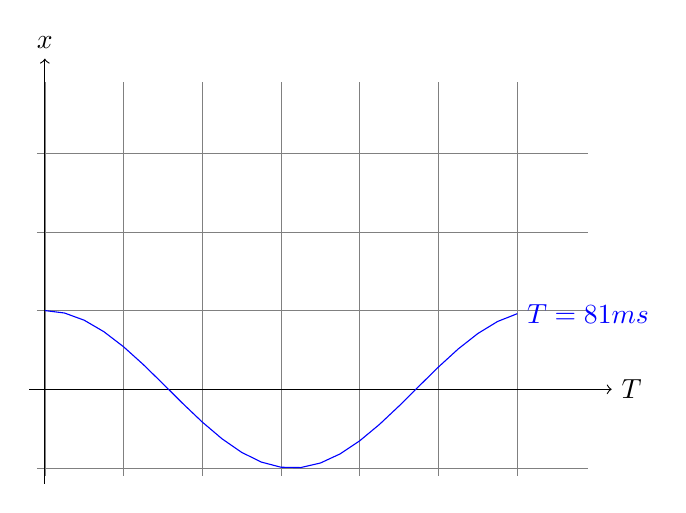
\begin{tikzpicture}[domain=0:6] 
	\draw[very thin,color=gray] (-0.1,-1.1) grid (6.9,3.9);
	\draw[->] (-0.2,0) -- (7.2,0) node[right] {$T$}; 
	\draw[->] (0,-1.2) -- (0,4.2) node[above] {$x$};
	\draw[color=blue]   plot (\x,{cos(\x r)})    node[right] {$T=81ms$}; 
\end{tikzpicture}\\
Prendendo l'esempio del pendolo
\begin{center}
	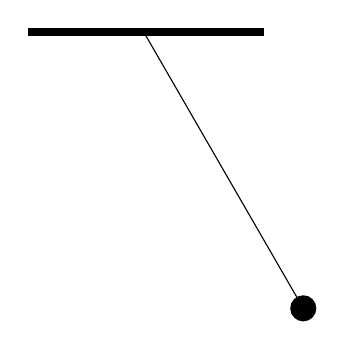
\begin{tikzpicture}
		% Support
		\fill (-1.5,0) rectangle(1.5,0.1);
		% Rod + Bob
		\draw (0,0) -- (-60:4) node[fill,circle](m){};
	\end{tikzpicture}
\end{center}
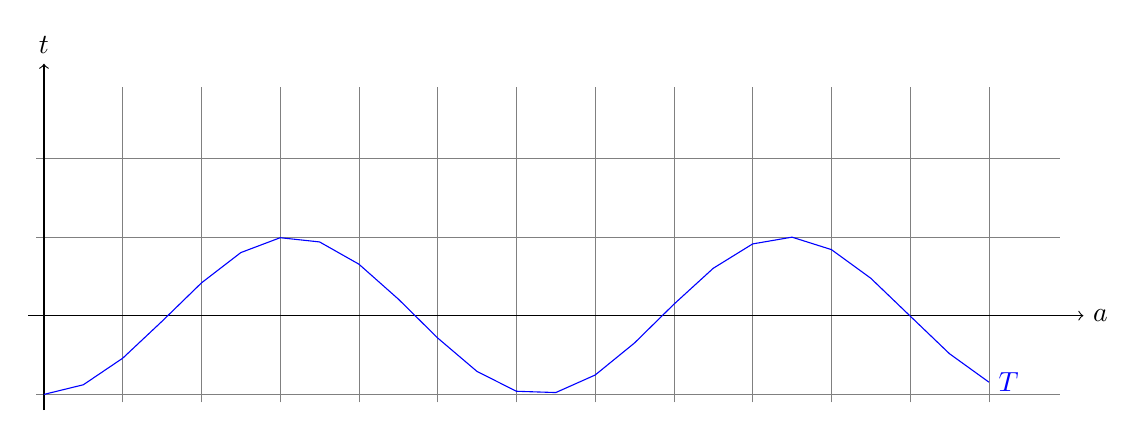
\begin{tikzpicture}[domain=0:12] 
	\draw[very thin,color=gray] (-0.1,-1.1) grid (12.9,2.9);
	\draw[->] (-0.2,0) -- (13.2,0) node[right] {$a$}; 
	\draw[->] (0,-1.2) -- (0,3.2) node[above] {$t$};
	\draw[color=blue]   plot (\x,{-cos(\x r)})    node[right] {$T$}; 
\end{tikzpicture}\\

